\documentclass[a4paper, 12pt]{article}
\usepackage[T2A]{fontenc}
\usepackage[utf8]{inputenc}
\usepackage[english,russian]{babel}
\usepackage{amsmath, amsfonts, amssymb, amsthm, mathtools, misccorr, indentfirst, multirow}
\usepackage{wrapfig}
\usepackage{graphicx}
\usepackage{subfig}
\usepackage{enumitem}
\usepackage{adjustbox}
\usepackage{pgfplots}
\usepackage{caption}

\usepackage{geometry}
\geometry{top=20mm}
\geometry{bottom=20mm}
\geometry{left=20mm}
\geometry{right=20mm}
\newcommand{\angstrom}{\textup{\AA}}
\begin{document}
	\begin{titlepage}
		\begin{center}
		МИНИСТЕРСТВО ОБРАЗОВАНИЯ И НАУКИ РОССИЙСКОЙ ФЕДЕРАЦИИ\\
		\footnotesize{Московский физико-технический институт}\\
		\footnotesize{(государственный университет)}\\
		\vfill
		{\LARGE
		\textbf{Исследование работы сдвигового регистра на цилиндрических магнитных доменах}\\
		}
		\vspace{1cm}
		Лабораторная работа по курсу\\
		тведотельная электроника
		\vfill
		\begin{flushright}
			Выполнил: студенты 654 группы.\\
			Нехаев А.С.\\
		\end{flushright}
		\vfill
		г. Долгопрудный\\
		\the\year\:год
		\end{center}
	\end{titlepage}
	\newpage
	\pagenumbering{arabic}
	\tableofcontents
	\newpage
	\section{Введение}
	\paragraph{Цель работы:}
	экспериментально рассмотреть процесс движения цилиндрических магнитных доменов, рассмотреть принцип работы запоминающего устройства на основе ЦМД.
	\subsection{Теоретическое введение}
	Ферромагнитный кристалл в отсутствие внешнего магнитного поля разбивается на области спонтанной намагниченности -- домены, в пределах которых намагниченность постоянна. В магнитоодноосных кристаллах границы между доменами параллельны некоторой оси симметрии кристалла -- оси легкого намагничивания.

	ЦМД является одной из возможных форм доменов. Равновесные состояния ЦМД определяются нулем вариации действия (или полной энергии). Уравнение равновесия сводится к таковому, состоящему из трех слагаемых, два из которых отвечают за сжатие ЦМД (обобщенная сила поверхностного натяжения на границах ЦМД и обобщенная сила взаимодействия намагниченности ЦМД и внешнего поля), и одно – за растяжение (обобщенная магнитостатическая сила). Решение этого уравнения выделяет некоторую область в пространстве линейных размеров (диаметров) и внешних полей $(d, H)$, соответствующую устойчивому состоянию ЦМД. Внешние поля $H$, направленные параллельно оси анизотропии кристалла, будем называть полями смещения $H_{\text{см}}$.

	Запоминающие устройства, основанные на ЦМД, используют наличие или отсутствие домена в некоторой области в качестве логических единицы и нуля соответственно. Для перемещения доменов с целью переноса информации в нужные области используются локальные магнитные поля, эффективно действующие на границу ЦМД. Для создания таких полей предназначены так называемые управляющие элементы, примером которых являются намагничиваемые внешним однородным управляющим полем (полем вращения) участки ферромагнитной пленки-аппликации.

	Под областью работоспособности элемента запоминающего устройства на ЦМД понимается множество пар значений полей смещения $H_{\text{см}}$ и вращения $H_{\text{вр}}$, при которых элемент функционирует без искажения информации (т.е. сохраняется доменная структура типа ЦМД).

	\section{Экспериментальная часть}
	Экспериментальная установка представлена микроскопом с установленными на предметном столике фрагментом сдвигового регистра и катушками для задания полей смещения и вращения. В поле зрения окуляра микроскопа находится часть массива хранения информации сдвигового регистра, и при различных значениях полей вращения и смещения наблюдается доменная структура сдвигового регистра (ЦМД, полосовые домены и проч.). Выставляя некоторые значения поля вращения, можно найти поля смещения, соответствующие коллапсу ЦМД и их превращению в полосовые домены, и, таким образом, определить границы области работоспособности представленного элемента. Поля вращения и смещения устанавливаются регулировкой тока в соответствующих катушках и определяются последующим переводом значений токов, снятых с амперметров, в значения магнитных полей.

	Сведем результаты измерений в таблицу:
	\newpage
	\begin{table}[!htb]
		\centering
		\caption{Результаты измерений полей коллапса и вырождения в полосовые домены.}
		\begin{tabular}{|c|c|c||c|c|c|}
			\hline
			$I_{\text{вр}}$, А & $I_{\text{вырождения}}$, А & $I_{\text{коллизии}}$, А & $H_{\text{вр}}$, э & $H_{\text{вырождения}}$, э & $H_{\text{коллизии}}$, э\\
			\hline
			0.98 & 0.63 & 0.96 & 49 & 69.3 & 105.6\\
			0.9 & 0.58 & 0.95 & 45 & 63.8 & 104.5\\
			0.8 & 0.59 & 0.92 & 40 & 64.9 & 101.2\\
			0.7 & 0.53 & 0.82 & 35 & 58.3 & 90.2\\
			0.6 & 0.58 & 0.79 & 30 & 63.8 & 86.9\\
			0.5 & 0.6 & 0.81 & 25 & 66 & 89.1\\
			0.4 & 0.6 & 0.75 & 20 & 66 & 82.5\\
			0.3 & 0.6 & 0.7	& 15 & 66 & 77\\
			\hline
		\end{tabular}
	\end{table}

	По полученным значениям построим график зависимости $H_{\text{см}}(H_{\text{вр}})$:
	\begin{figure}[!htb]
		\centering
		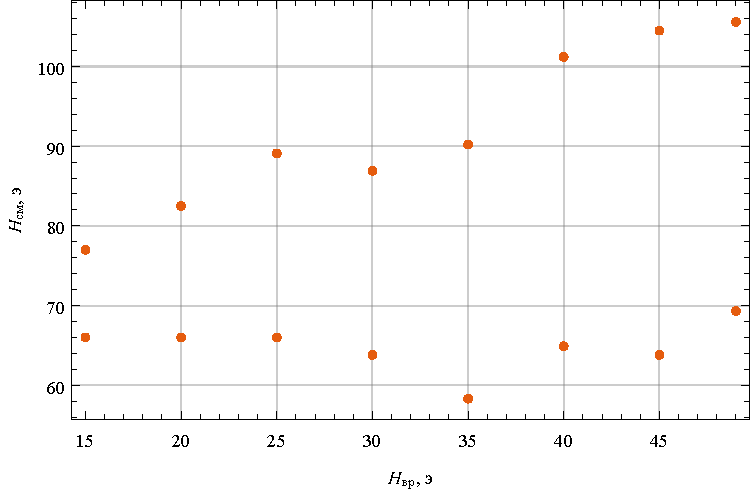
\includegraphics[scale=1]{plot.pdf}
		\caption{Область работоспособности сдвигового регистра.}
		\label{fig1}
	\end{figure}
	\section{Аппроксимация полученных значений}
	Представим эллипс в виде уравнения для кривой второго порядка:
	\begin{equation*}
		a_{11}x^2+a_{22}y^2+2a_{12}xy+2a_{13}x+2a_{23}y+a_{33}=0.
	\end{equation*}
	Используя экспериментальные значения, проведем аппроксимацию при помощи модели линейной регрессии и при подставновке полученных коэффициентов получим уравнение:
	\begin{equation*}
		0.318136 x^2-0.984878 x y+45.3094 x+y^2-124.066 y+4052.35=0.
	\end{equation*}
	Приведем таблицу со статистическими значениями полученных коэффициентов:
	\newpage
	\begin{table}[!htb]
		\centering
		\begin{tabular}{|c||c|c|c|c|}
			\hline
			 & Estimate & Standard Error & t-Statistic & P-Value\\
			\hline
			1 & -4052.35 & 542.265 & -7.47301 & 0.0000124107 \\
 			a & -0.318136 & 0.237607 & -1.33892 & 0.20761 \\
			b & -45.3094 & 17.3549 & -2.61075 & 0.0242249 \\
			c & 124.066 & 7.49768 & 16.5473 & $4.04\cdot 10{-9}$ \\
			d & 0.492439 & 0.0940312 & 5.23697 & 0.000278118 \\
			\hline
		\end{tabular}
	\end{table}

	По полученным значениям построим график:
	\begin{figure}[!htb]
		\centering
		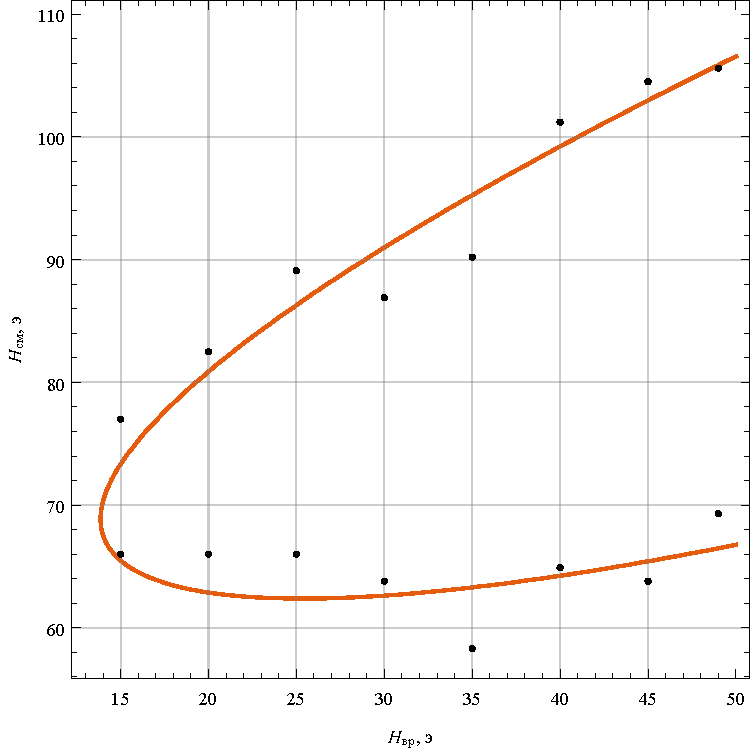
\includegraphics[scale=1]{plot2.pdf}
		\caption{Область работоспособности линейного участка элемента продвижения}
		\label{fig2}
	\end{figure}
	\section{Вывод}
	В ходе работы нам удалось рассмотреть процесс движения ЦМД в сдвиговом регистре, найти его область работоспособности; полученные результаты приведены в виде графика на рисунке \ref{fig1}, их вид соответствует теоретической модели, что продемонстрировано на рисунке \ref{fig2}.
\end{document}